\documentclass[../main.tex]{subfiles}


\begin{document}

\section{Metrické prostory}
\subsection{Definice metrického prostoru}

\begin{definition}[Metrický prostor]
	Nechť $X$ je množina,  $d: X \times X \rightarrow \mathbb{R}$ funkce t. ž. platí:
	
	\begin{itemize}
	\item{$\forall x,y \in X : d(x,y) \geq 0, \quad d(x,y) = 0 \iff x = y$ }
	\item{$\forall x,y \in X : d(x,y) = d(y,x)$}
	\item{$\forall x,y \in X : d(x,z) \leq d(x,y) + d(y,z)$ (trojúhelníková nerovnost)}
	\end{itemize}
	pak $(X,d)$ je metrický prostor.
\end{definition}

\begin{example}
	Zde je několik metrických prostorů:
	\begin{align*} 
	    (\mathbb{R}, |x-y|) &,\\
	    (\mathbb{C},|x-y|) &,\\
	    (G,d) &, G \text{ je orientovaný souvislý graf, } d \text{ je délka nejdelší cesty}
	\end{align*}%
	Pozor: trojúhelníková nerovnost v $(\mathbb{C}, |x-y|)$ není tak triviální jako v $\mathbb{R}$.
\end{example}

\begin{definition}[Euklidovský prostor $\mathbb{E}_n$]
Definujeme jako metrický prostor $(\mathbb{R}^n,d)$, kde $d$:
\[d((x_1,...,x_n),(y_1,...,y_n)) = \sqrt{\sum_i(x_i-y_i)^2}\]
Pro nás zvlášť důležitý, známý v podobě vektorového prostoru $\mathbb{R}^n$ se skalárním součinem $\langle \textbf{u} | v \rangle$ a normou
$\|\textbf{u}\| = \sqrt{\textbf{uu}}$ a vzdáleností $d(\textbf{u},v) = ||\textbf{u}-v||$
\end{definition}

\begin{definition}[Diskrétní prostor]
	Definujeme jako $(X,d)$, kde $d(x,y) = 1$ pro $x \neq y$
\end{definition}

\begin{definition}[Podprostor]
	Buď $(X, d)$ metrický prostor. Pak $(Y, d')$ je podprostor, kde $Y \subseteq X$ a $\forall x,y \in Y : d'(x,y) = d(x,y)$.
\end{definition}

\begin{definition}[Spojité zobrazení]
	$f \colon (X,d) \to (Y, d')$ je spojité zobrazení, pokud
	\[ \forall x, y \in X, \forall \varepsilon > 0 \exists \delta > 0:
	d(x,y) < \delta \Rightarrow d'(f(x), f(y)) < \varepsilon \]
\end{definition}

\subsection{Triviality}

\begin{definition}[Identické zobrazení]
	$f(x) = x$ je spojité zobrazení
	\[ (X,d) \to (X,d) \]
\end{definition}

\begin{definition}[Vložení podprostorů]
	je spojité zobrazení
	\[ f_1\colon (X_1,d_1)\times(X_2,d_2) \rightarrow (X_1,d_1) \]
	\[\forall x\in X_1 \forall y \in X_2 : f_1(x,y) = x\]
	\[f_2 \colon (X_1,d_1)\times(X_2,d_2) \rightarrow (X_2,d_2)\]
	\[\forall x\in X_1 \forall y \in X_2 : f_2(x,y) = y\]
	\[\text{obecně pro } j=1,...,n \text{ máme}\]
	\[f_j\colon\prod^n_{i=1}(X_i,d_i)\rightarrow(X_j,d_j)\]
	\[f_j(x_1,x_2,...,x_n) = x_j\]
\end{definition}

\begin{definition}[Konvergence]
	Posloupnost $(x_n)_n$ v metrickém prostoru $(X, d)$ konverguje k $x \in X$, pokud
	$$\forall \varepsilon > 0\ \exists n_0: \forall n \ge n_0: d(x_n, x) < \varepsilon$$
\end{definition}

\subsection{Věty o metrických prostorech}

\begin{theorem}[Složení spojitých zobrazení je spojité]
	Pokud jsou $f: (X_1,d_1) \to (X_2, d_2)$ a $g: (X_2,d_2) \to (X_3, d_3)$ spojité, pak i
	\[ g \circ f: (X_1,d_1) \to (X_3,d_3) \] je spojité.
\end{theorem}

\begin{theorem}[Věta o konvergenci]
	Zobrazení $f: (X_1,d_1) \rightarrow (X_2,d_2)$ je spojité právě když pro každou konvergentní $(x_n)_n$ v $(X_1,d_1)$ 
	posloupnost $(f(x_n))_n$ konverguje v $(X_2,d_2)$ a platí $\lim_n f(x_n) = f(\lim_n x_n)$.
\end{theorem}

\begin{proof}
	\hfill %https://latex.org/forum/viewtopic.php?t=14853
	\begin{itemize}
		\item[$\Rightarrow \phantom{\lnot}$] Buď $f$ spojitá a nechť $\lim_nx_n = x$. Pro $\varepsilon > 0$ volme ze spojitosti $\delta > 0$
		tak, aby $d_1(x,y) <\delta \implies d_2(f(x),f(y)) <\varepsilon$.
		Podle definice konvergence posloupnosti existuje $n_0$ takové, že pro $n \ge n_0$ je $d_1(x_n,x) < \delta$. Tedy je-li $n \ge n_0$
		máme $d_2(f(x_n),f(x)) < \varepsilon$ a potom $\lim_n f(x_n) = f(\lim_n x_n)$.
		\item[$\lnot \Rightarrow  \lnot$] Nechť $f$ není spojitá.
		Potom existují $x \in X_1$ a $\varepsilon_0 > 0$ takové, že pro každé $\delta > 0$ existuje $x_\delta$ takové, že
		$$d_1(x, x_\delta) < \delta \qquad \text{ale} \qquad d_2(f(x), f(x_\delta) \ge \varepsilon_0$$
		Položme $x_n = x_{1/n}$. Potom $\lim_n x_n = x$ ale $(f(x_n))_n$ nemůže konvergovat k $f(x)$.
	\end{itemize}
\end{proof}



\subsection{Okolí, množiny, uzávěry}
\begin{definition}[Okolí]
	Nechť $(X,d)$ je metrický prostor, $x\in X$, pak
	$$\Omega (x,\varepsilon) = \{ y\ |\ d(x,y) < \varepsilon \}$$
	Formulaci $\Omega (x,\varepsilon)$ se říká otevřená koule s poloměrem $\varepsilon$ okolo $x$.
\end{definition}

\begin{example} [Použití okolí]
	$"\textrm{U je okolí } x" \equiv \exists \varepsilon > 0, \Omega (x,\varepsilon) \subseteq U $
\end{example}

\begin{definition}[Otevřená množina]
	$U \subseteq (X,d)$ je otevřená, pokud je okolím \textit{každého} svého bodu.
\end{definition}

\begin{definition}[Uzavřená množina]
	$V \subseteq (X,d)$ je uzavřená, pokud $\forall (x_n)_n \subseteq V$ je konvergentní
	v $X$ a $\lim_n x_n \in V$.
\end{definition}

\begin{definition}[Vzdálenost od množiny]
	Nechť $(X,d)$ je metrický prostor, $A \subseteq X, x\in X$, pak vzdálenost bodu $x$ od množiny $A$ je
	\[d(x,A) = \inf\{d(x,a)\mid a \in A\}\]
\end{definition}

\begin{definition}[Uzávěr]
	$\overline{A} : \{x \mid d(x,A) = 0\}$
\end{definition}

\subsection{Vzory a obrazy}
Pro zbytek sekce nechť $f: X \rightarrow Y, A \subseteq X, B \subseteq Y$.

\begin{definition}[Obraz]
	Obraz podmnožiny $A\subseteq X$ v $Y$:
	\[f[A] = \{f(x) \mid x \in A\}\]
\end{definition}

\begin{definition}[Vzor]
	Vzor podmnožiny $B\subseteq Y$ v $X$:
	\[f^{-1}[B] = \{x \mid x \in X: f(x) \in B\}\]
	\[X \underset{f^{-1}[-]}{\stackrel{f[-]}{\rightleftarrows}} Y\]
	Pozor, $f^{-1}$ má dva významy:
	\begin{itemize}
		\item inverze $f^{-1}:Y \rightarrow X$, nemusí existovat
		\item část v symbolu $f^{-1}[-]$, má smysl vždy
	\end{itemize}
\end{definition}

\begin{lemma}[Vztahy vzorů a obrazů]
	\[f[A] \subseteq B \equiv A \subseteq f^{-1}[B],\]
	\[f[f^{-1}[B]] \subseteq B\]
	\[f^{-1}[f[A]] \supseteq A\]
\end{lemma}

\begin{theorem}[Vlastnosti zobrazení mezi metrickými prostory]
	Buďte $(X_1, d_1)$ a $(X_2, d_2)$ metrické prostory a buď zobrazení $f: X_1 \to X_2$. Následující tvrzení
	jsou potom ekvivalentní:
	\begin{enumerate}
	    \item $f$ je spojité.
	    \item $\forall x \in X_1$ a $\forall$ okolí $V$ bodu $f(x)$ existuje okolí $U$ bodu $x$ takové, že
	        $f[U] \subseteq V$.
	    \item $\forall$ otevřenou $U$ v $X_2$ je vzor $f^{-1}[U]$ otevřený v $X_1$.
	    \item $\forall$ uzavřenou $A$ v $X_2$ je vzor $f^{-1}[A]$ uzavřený v $X_1$.
	    \item $\forall A \subseteq X_1$ je $f[\overline{A}] \subseteq \overline{f[A]}$
	\end{enumerate}
\end{theorem}

\subsection{Ekvivalence metrik}

\begin{definition}[Ekvivalentní metriky]
	Metriky $d_1, d_2$ na téže množině jsou ekvivalentní, pokud $\mathrm{id}_X : \left(X, d_1\right) \to (X, d_2)$ je homeomorfismus. Získáme tím prostor, ve kterém jsou všechny topologické záležitosti (spojitost, uzavřenost, \ldots) zachovány.
\end{definition}


\begin{definition}[Silně ekvivalentní metriky]
	Metriky $d_1$ a $d_2$ na téže množině jsou silně ekvivalentní, pokud
	\[\exists \alpha , \beta > 0: \alpha d_1(x,y) \leq d_2(x,y) \leq \beta d_1(x,y)\]
\end{definition}

%%%%%%%%%%%%%%%%%%%%%%%%%%%%%%%%%%%%%%%%%%%%%%%%%%%%%%%%%%%%%%%%%%%%%%%%%%%%%%%%%%%%%%%%%%%%%%%%%%%%%%%%%
\subsection{Součiny}

\begin{definition}[Součin]
	Pro $(X_1,d_i), i = 1,...,n$ definujeme na kartézském součinu $\prod^n_{i=1}X_i$ metriku
	\[d((x_1,...,x_n),(y_1,...,y_n)) = \max_i d_i(x_i,y_i)\]
	Získaný
	\[\prod^n_{i=1}(X_i,d_i)\]
	se nazývá součin prostorů $(X_i, d_i)$. Píše se též 
	\[(X_1,d_1) \times \cdots \times (X_n,d_n).\]
\end{definition}

%%%%%%%%%%%%%%%%%%%%%%%%%%%%%%%%%%%%%%%%%%%%%%%%%%%%%%%%%%%%%%%%%%%%%%%%%%%%%%%%%%%%%%%%%%%%%%%%%%%%%%%%%
\subsection{Věta o spojitých zobrazeních}
\begin{theorem}[O spojitých zobrazeních]
	\hfill
	\begin{enumerate}
	\item Projekce $p_j = ((x_i)_i \mapsto x_j) : \prod^n_{i=1}(X_i,d_i) \rightarrow (X_j,d_j)$ jsou spojitá zobrazení.
	
	\item Buďte $f_j:(Y,d') \rightarrow (X_j,d_j)$ libovolná spojitá zobrazení. Potom jednoznačně určené zobrazení 
	$f:(Y,d') \rightarrow \prod^n_{i=1}(X_i,d_i)$ splňující $p_j \circ f = f_j$, totiž zobrazení definované předpisem
	$f(y) = (f_1(y),...,f_n(y))$, je spojité.
	\end{enumerate}
\end{theorem}

\begin{intuition}
	Jak to vypadá:
	\begin{center}
	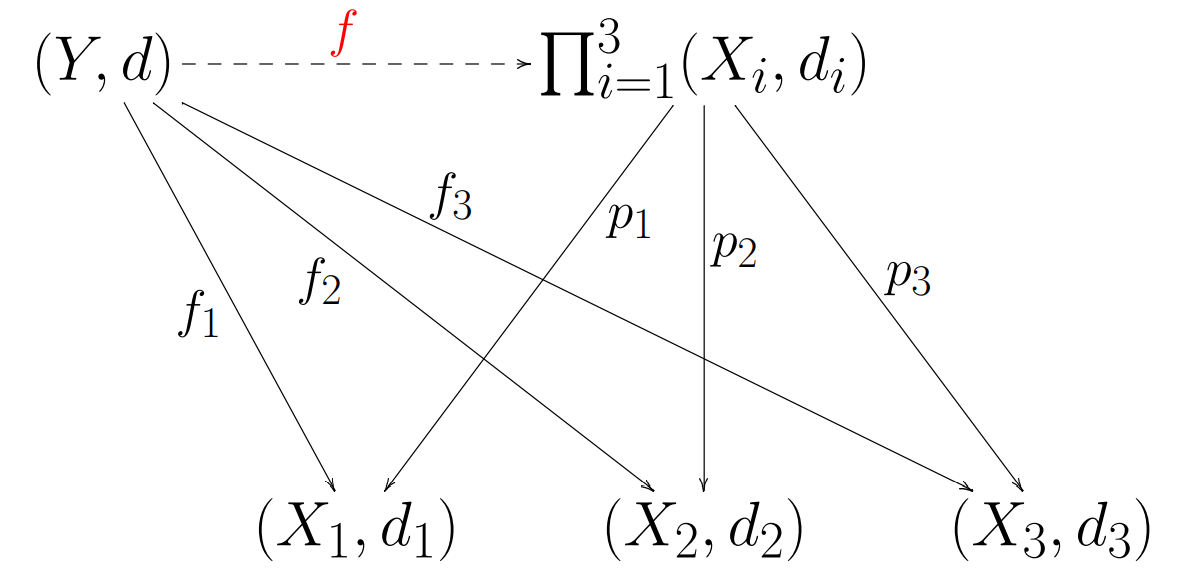
\includegraphics[width=9cm,height=4.8cm]{ipkm.png}
	\end{center}
	Tedy pokud víme, že $(x_1,x_2,x_3)\in \prod (x_i,d_i)$, Pak
	\[f(y) = (f_1(y),f_2(y),f_3(y))\]
	\[(p_1\circ f)(y) = p_1(f(y)) = p_1(f_1(y),f_2(y),f_3(y))=f_1(y)\]
	\[(p_2\circ f)(y) = ... = f_2(y)\]
	\[(p_3\circ f)(y) = ... = f_3(y)\]
	Existuje přesně jedno $f$ takové, že 
	\[p_i \circ f = f_i\]
	a je spojité.
\end{intuition}

\end{document}
